\documentclass{article}
\usepackage{tikz}

\begin{document}

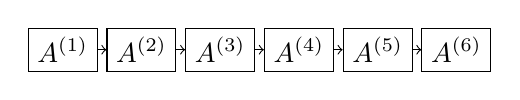
\begin{tikzpicture}[node distance=1cm]
    \node[draw] (A1) {$A^{(1)}$};
    \node[draw, right of=A1] (A2) {$A^{(2)}$};
    \node[draw, right of=A2] (A3) {$A^{(3)}$};
    \node[draw, right of=A3] (A4) {$A^{(4)}$};
    \node[draw, right of=A4] (A5) {$A^{(5)}$};
    \node[draw, right of=A5] (A6) {$A^{(6)}$};

    \draw[->] (A1) -- (A2);
    \draw[->] (A2) -- (A3);
    \draw[->] (A3) -- (A4);
    \draw[->] (A4) -- (A5);
    \draw[->] (A5) -- (A6);
\end{tikzpicture}

\end{document}